%        File: Proposal.tex
%     Created: Thu Aug 25 12:00 PM 2016 E
% Last Change: Thu Aug 25 12:00 PM 2016 E
%
% arara: pdflatex
% arara: biber
% arara: pdflatex
% arara: pdflatex
\documentclass[letterpaper,12pt]{article}

\usepackage[
margin=1in
]{geometry}
\usepackage[backend=biber,style=authoryear-comp,useprefix=false]{biblatex}

\usepackage{stmaryrd}
\usepackage[]{amsmath}
\usepackage{amsfonts}
\usepackage{amssymb}
\usepackage{mathtools}
\usepackage{forest}
\usepackage{tabularx}
\usepackage{linguex}
\usepackage{centernot}
\usepackage{todonotes}
\usepackage{titling}
\useforestlibrary{linguistics}

\forestset{tree defaults/.style={for tree={parent anchor=south, child anchor=north},every tree node/.style={align=center,anchor=north},level/.style={sibling distance=50mm/#1},baseline}}

\forestset{en/.style={parent anchor=center, child anchor=center}}
\forestset{em/.style={parent anchor=north west, child anchor=north west}}
\forestset{el/.style={parent anchor=north, child anchor=north}}

\usetikzlibrary{positioning}
\usetikzlibrary{calc}
\usetikzlibrary{arrows}
\usetikzlibrary{decorations.markings}
%\DeclareNameFormat{labelname:poss}{% Based on labelname from biblatex.def
%  \ifcase\value{uniquename}%
%  \usebibmacro{name:last}{#1}{#3}{#5}{#7}%
%  \or
%  \ifuseprefix
%  {\usebibmacro{name:first-last}{#1}{#4}{#5}{#8}}
%  {\usebibmacro{name:first-last}{#1}{#4}{#6}{#8}}%
%  \or
%  \usebibmacro{name:first-last}{#1}{#3}{#5}{#7}%
%  \fi
%  \usebibmacro{name:andothers}%
%  \ifnumequal{\value{listcount}}{\value{liststop}}{'s}{}
%}
%
%\DeclareFieldFormat{shorthand:poss}{%
%  \ifnameundef{labelname}{#1's}{#1}
%}
%
%\DeclareFieldFormat{citetitle:poss}{\mkbibemph{#1}'s}
%
%\DeclareFieldFormat{label:poss}{#1's}
%
%\newrobustcmd*{\posscitealias}{%
%  \AtNextCite{%
%    \DeclareNameAlias{labelname}{labelname:poss}%
%    \DeclareFieldAlias{shorthand}{shorthand:poss}%
%    \DeclareFieldAlias{citetitle}{citetitle:poss}%
%    \DeclareFieldAlias{label}{label:poss}
%  }
%}
%
%\newrobustcmd*{\posscite}{%
%  \posscitealias%
%  \textcite
%}
%
%\newrobustcmd*{\Posscite}{\bibsentence\posscite}
%
%\newrobustcmd*{\posscites}{%
%  \posscitealias%
%  \textcites
%}

\newcommand\quelle[1]{{%
  \unskip\nobreak\hfil\penalty50
  \hskip2em\hbox{}\nobreak\hfil#1%
  \parfillskip=0pt \finalhyphendemerits=0 \par
}
}

\newcommand{\figex}{\refstepcounter{ExNo}\theExNo\hspace{\Exlabelsep}}

\newcounter{DerivStep}

\newcommand{\hxp}{$\left\{ \text{X, YP} \right\}$}
\newcommand{\hh}{$\left\{ \text{X, Y} \right\}$}
\newcommand{\xpyp}{$\left\{ \text{XP, YP} \right\}$}
\bibliography{Thesis}
\linespread{1.3}

\title{Explaining the Resultative Parameter\\{\large Thesis Proposal}}
\author{Dan Milway}
\begin{document}
\maketitle

\section{Introduction}
The promise of generative syntax is that, given fixed innate grammatical principles, unlearnable and seemingly deep variation can be derived from learnable surface variation.
In current minimalist theories of syntax, the locus of variation in the lexicon, as expressed succinctly by \citeauthor{baker2008microparameter}'s (\citeyear{baker2008microparameter}) Borer-Chomsky Conjecture, given below in \Next.
\ex. The Borer-Chomsky Conjecture\\
All parameters of variation are attributable to differences in the features of particular items (e.g., the functional heads) in the lexicon. \hfill \parencite{baker2008microparameter}

This conjecture follows from various theoretical and empirical findings throughout the history of generative grammar, but has not yet been shown to be explanatory.
Consider the correlation between obligatory predicative adjective agreement and the impossibility of adjectival resultatives \parencite{kratzer_building_2004}, as can be observed in the differences between French and German.
In both languages, attributive adjectives agree for number and gender (and case, in German) with the nominals they modify. 
The languages differ with respect to predicative agreement, however.
German disallows agreement on predicative adjectives, while French requires it.
\ex. French 
\ag. la grand *(-e) femme\\
The tall \textsc{~~agr} woman(Fem)\\
``the tall woman''
\bg. La femme est grand *(-e).\\
the woman(fem) is tall \textsc{~~agr}\\
``The woman is tall.''
\z.

\ex. German 
\ag. die gro\ss{} *(-e) Frau\\
the tall \textsc{~~agr} woman\\
``the tall woman''
\bg. Die Frau ist gro\ss{} (*-e).\\
the woman(fem) is tall \textsc{~~agr}\\
``The woman is tall''
\z.

These patterns, being observable on the surface, are in principle learnable from the primary linguistic data (PLD).

The languages also differ in whether they allow resultative interpretations of secondary predicates (SPs).
French (along with other Romance languages) allows only depictive SPs, while German (along with other Germanic languages) allows both depictive and resultative SPs.
\ex.Germanic
\a. English
\a. I ate the fish raw. (depictive)
\b. I hammered the metal flat. (resultative)
\z.
\b.German 
\ag. Er i\ss{}t das Fleisch roh. \parencite{muller2004analysis}\\
He eats the meat raw { }\\
``He's eating the meat raw.'' (depictive)
\bg. Wir haben die teekanne leer getrunken. \parencite{kratzer_building_2004}\\
we have the teapot empty drink.\textsc{part} { }\\
``We drank the teapot dry.''(resultative)
\z.
\z.

\ex. Romance
\a. French
\ag. Pierre mange la viande crue. \parencite{legendre1997secondary}\\
Pierre eat.3sg the.fem meat raw.fem { }\\
``Pierre ate the meat raw'' (depictive)
\bg.* Il a march\'e les jambes raides. \parencite{washio1997resultatives}\\
He has walked the legs stiff { }\\
``He walked his legs off.'' (resultative)
\z.
\b. Italian
\ag. l' ho mangiato crudo.\\
3sg \textsc{aux}.1sg eaten raw\\
``I ate it raw'' (depictive)
\bg.* l' ho bevuto vuoto.\\
3sg \textsc{aux}.1sg drank empty\\
``I drank it dry'' (resultative)
\z.
\z.

Since the variation demonstrated in \LLast and \Last has to do with the meanings assigned to expressions rather than surface properties of the expressions, such variation is not, in principle, learnable from the PLD.

So, we have two types of variation (one shallow and learnable, one deep and unlearnable) which seem to be correlated with each other (predicative adjective agreement $\leftrightarrow$ *adjectival resultatives).
Given the Borer-Chomsky Conjecture, then, it is a reasonable hypothesis that the unlearnable variation follows somehow from the learnable variation.
That is, the lack of predicative adjective agreement makes adjectival resultatives possible in German, while its presence in French disallows them.

The hypothesis that such disparate phenomena might be linked should surprise no-one familiar with minimalist theorizing.
In this thesis, I propose to explore the nature of such a link.
Specifically, I will argue that Chomsky's (\citeyear{chomsky2013problems,chomsky2015problems}) recent label theory, taken to its logical conclusion, explains the link between adjectival morphology and resultative SPs.


\subsection{Previous Answers}
The puzzle of the resultative parameter has been approached from two directions.
One approach, found in the work of \textcite{harley2005how,folli2006licensing,ramchand2008verb,tungseth2008verbal}, among others, first asks how we might represent resultatives syntactically and then asks what a language's lexicon would have to look like in order to block the structures underlying resultatives.
Such an approach also tends to assume that lexical verbs are decomposable into several heads bearing primitive conceptual features (\textsc{Process}, \textsc{Manner}, \textsc{Result}, \textsc{Path}, \textit{etc.}) in the spirit of \textcite{hale1993argument}.
In my first generals paper \parencite[][pp 30-32]{milway2015generals}, I argue that Ramchand's (\citeyear{ramchand2008verb}) particular proposal, which is perhaps the most fully realized and coherent proposal of this type, falls short of providing a syntactic analysis of the resultative parameter.
Furthermore, none of the work in this approach explicitly addresses the question of how such variation could be acquired, rather, they implicitly assume that it can be acquired.

The second approach to the resultative parameter, found in the work of \textcite{snyder1995language,snyder2001nature,roeper2002learnability,beck2001complex}, starts with the acquisition question.
In his 1995 dissertation, Snyder presents evidence from child language data that the acquisition of endocentric compounding is correlated with that of resultatives, and argues that they both follow from a single syntactic parameter, given below in \Next.
\ex. \textbf{The Compounding Parameter} \parencite{snyder2001nature}\\ 
The grammar \{disallows*, allows\} formation of endocentric compounds during the syntactic derivation. [*unmarked value] 

While an interesting description, this work also falls short of an explanation of the resultative parameter because it merely identifies a correlation between two phenomena but does not attempt to establish a causal link between them.
\textcite{kratzer_building_2004} attempts to describe such a link, but for reasons discussed in my first generals paper \parencite[][pp 32-34]{milway2015generals}, also falls short of explanatory adequacy.

My thesis will be an attempt to unify the two approaches. 
Such a unification, however, will require significant revision of the logic used in each approach.
I will discuss the revised logic in the following section.

\section{Towards an explanation of the resultative parameter}\label{sec:outline}

The first line will be an attempt to formalize the surface variation associated with the resultative parameter.
\textcite{snyder2001nature,roeper2002learnability,kratzer_building_2004} and others identify the (un)availability of productive compounding as the relevant surface variation, while \textcite{haider2016predicting} identifies the (un)availability of particle verb constructions as the culprit.
My previous investigation of particle verbs \parencite[][included as an appendix]{milway2013forum} suggests that compounding and particle verbs are related, so I will provisionally assume that the compounding parameter subsumes the particle verb parameter.\footnote{
  This assumption will be revised in later sections of the thesis.
}
This variation is typically expressed as parameters of the grammar, such as Snyder's Compounding Parameter below.
\ex. \textbf{Compounding Parameter} \parencite{snyder2001nature}\\ 
The grammar \{disallows*, allows\} formation of endocentric compounds during the syntactic derivation. [*unmarked value] 

Under standard minimalist assumptions, \Last would be considered a descriptive/typological statement in need of theoretical explanation.

The first step towards such an explanation is to rephrase \Last with the Borer-Chomsky Conjecture in mind.
If we consider an I-language, L, to be the pair of a variable lexicon, Lex$_\text{L}$, and a fixed Universal Grammar, UG, then we can restate the Compounding Parameter as in \Next.
\ex. \textbf{Compounding Parameter} (revised):\\
The lexicon of an I-language, L, is such that principles of UG \{disallow*, allow\} formation of endocentric compounds during a syntactic derivation in L. [*unmarked value]

From this formulation, the next step is to investigate exactly how endocentric compounds are derived syntactically and how they might be blocked.
If this investigation is done by holding the principles of UG constant, then we will have arrived at a characterization of those properties of the lexicon that are linked to the Compounding Parameter.

The second line of inquiry will investigate resultative structures directly, how they are derived, and how they are blocked.
As with the first line of inquiry, the goal of this line will be to identify the lexical properties that determine whether or not a given I-language generates resultatives.
If the correlation between compounding and resultatives is not a coincidence, the properties identified by this line of inquiry should be identical to those identified by the first line of inquiry.

The situation I hope to describe, schematized below in \Next,  will be a class of lexicons defined by a single shared property or set propertiesn which is associated in principle with both endocentric compounding (making it learnable from the PLD) and adjectival resultatives. 
\begin{figure}[h]
  \figex
  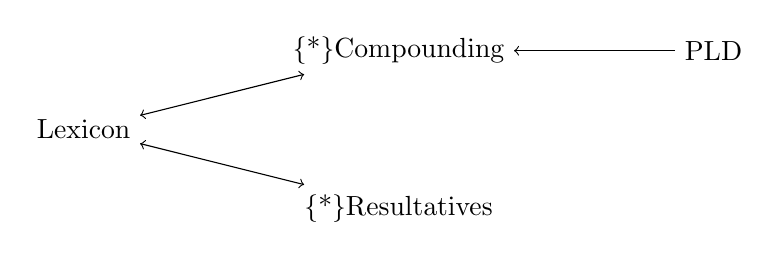
\begin{tikzpicture}[baseline]
    \node (lex) at (0,-1) {Lexicon};
    \node (comp) at (4,0) {\{*\}Compounding};
    \node (res) at (4,-2) {\{*\}Resultatives};
    \node (pld) at (8,0) {PLD};
    \draw [<->] (lex)--(comp);
    \draw [<->] (lex)--(res);
    \draw [->] (pld)--(comp);
  \end{tikzpicture}
  \label{fig:ParameterModel}
\end{figure}

\section{Sharpening the Question}\label{sec:result analysis}
A more precise definition of resultatives is needed to proceed in this study.
Resultative clauses  contain two distinct predicates (Pred1$\neq$Pred2) which share an argument, in which the primary predicate is construed as the cause of the secondary.
Each of these properties that define resultatives (argument sharing and ``causativity'') is quite common and neither is sufficient for resultatives.
Depictives such as those in \Next, which seem to occur in all languages, show argument sharing without ``causativity''.
\ex. \textbf{Depictives}
\a. Mary left angry. (Mary was angry.)
\b. Bill ate the fish raw. (The fish was raw.)
\b. Jamie swam the race naked. (Jamie was naked.)
\z.

So, the clause \textit{Mary left angry} means that the two eventualities, the event $e$ of Mary leaving and the state $s$ of Mary being angry, are stand in either an identity ($e=s$) or containment ($e\leq s$) relation rather than a causal relation.

``Causativity'', broadly construed, is even more prevalent in language.
Every instance of a sentence with an agent encodes ``causativity''.
For example, the clause \textit{John ironed the shirt} means that John acted in such a way as to cause the shirt to be ironed.

English-type languages, then, generate clauses in which a single argument is shared between two predicates which are in a ``causative'' relation.
French-type languages, on the other hand, do not generate clauses with both properties.
This means that an explanation of the parametric split between English- and French-type languages needs three components.
First, it requires a theory of argument sharing.
Second, it must include a theory of how relations between predicates are established.
Finally, it must show that, for a given language, there is some component of the primary lingustic data which determines whether the two phenomena are compatible.

\subsection{What is Argument Sharing}
First, Lets consider cases of argument sharing, which, semantically speaking, is a situation in which one entity is interpreted as being a participant in multiple distinct events expressed by a single utterence.
A familiar type of argument sharing is control sentences such as \Next, in which Alice is both the holder of the wanting attitude and the agent of the non-actual winning event.
\ex.\label{ex:Control} Alice$_i$ wants $ec_i$ to win.

Other instances of argument sharing are seen in parasitic gaps, and depictives as in \Next and \NNext, respectively.

\ex. Who$_i$ did you discuss $ec_i$ without meeting $ec_i$?

\ex. Monica left angry.

$\Theta$-roles are the syntactic analogue of the semantic predicate-argument relation.
If an entity is semantically interpreted as the argument of a predicate, then the phrase that encodes that entity is $\Theta$-marked by the head or phrase that encodes the predicate.
Following a basic minimalist assumption -- the Theta-Role Assignment Principle (TRAP) \parencite{hornsteinetal2005understanding} -- $\Theta$-roles are assigned upon merge, and, following a more controversial assumption -- the Uniformity of Theta Assignment Hypothesis (UTAH) \parencite{baker1988incorporation}-- there is a mapping between $\Theta$-roles and syntactic positions.
This means, for example, that a DP is interpreted as the Theme of a verb iff it is merged as the complement of that verb.

I will be making two non-standard assumptions about $\Theta$-roles.
First, I assume that DPs can receive multiple $\Theta$-roles, or in other words, I do not assume the $\Theta$ criterion.
This assumption is the basis for Hornstein's (\citeyear{hornstein1999movement,hornstein2009theory}) Movement Theory of Control, and the justifications I discuss below are adapted from Hornstein's justifications.
There are two justifications for this assumption, one metatheoretical and the other theoretical.
The metatheoretical argument is based on the method of theory building that characterizes the minimalist program.
Theories are built by identifying virtual conceptual necessities (VCNs) which are taken to be axioms of the theory.
A proposed principle or theoretical construct can be admitted to the theory in one of two ways:
Either it is shown to follow logically from VCNs or it is argued to be a VCN.
In current syntactic theory, the set of VCNs is restricted to a lexicon, a structure building operation (merge) and the interfaces with other cognitive modules (the sensorimotor and conceptual-intentional interfaces).
Since the $\Theta$-criterion is not a member of this set, its existence, rather than its nonexistence, must be argued for.
In other words, the burden of proof is on those who would propose the $\Theta$-criterion rather than those who reject it.

The $\Theta$-criterion was originally proposed as a constraint in GB syntax that held at D-Structure. 
It stated that every $\Theta$-role must be assigned to exactly one argument and every argument be assigned exactly one $\Theta$-role.
Since D-Structure has been eliminated from the theory, then if the $\Theta$-criterion does hold, it must hold at one of the interfaces, and since $\Theta$-roles are essentially semantic it would presumably hold at the CI-interface.
We must, tehrefore, ask how the $\Theta$-criterion would be formulated as a constraint on CI legibility.

To do so, let's consider a concrete case.
Compare the two possible structures for an instance of control in \Next.
\ex.
\a. Richard$_i$ wanted [PRO$_i$ to laugh].
\b. Richard$_i$ wanted [$\langle$Richard$_i\rangle$ to laugh].

The structure in \Last[a], with PRO, obeys the $\Theta$-criterion, and the one in \Last[b] violates it, but both map to the same logical form, given in \Next.
\ex. $\exists e [\text{Wanted}(e)(\textbf{r}) \& \text{Laugh}(e) \& \textsc{Agent}(e)(\textbf{r})]$

The $\Theta$-criterion would then amount to a stipulation that \LLast[a] is good and \LLast[b] is bad.
So far, I have found no need for such a stipulation.

The second non-standard assumption is the particular version of UTAH I use.
\textcite{baker1988incorporation} argues for the following mapping of $\Theta$-roles to structural position.
Agents are asssociated with Spec Voice, Themes with Spec V, and Goals with Comp V as in \Next, below.
\ex.\label{fig:BakerUTAH}
  {\small
\begin{forest}
  nice empty nodes,sn edges,baseline
  [VoiceP
    [\textsc{Agent}]
    [Voice$^\prime$
      [Voice]
      [VP
	[\textsc{Theme}]
	[V$^\prime$
	  [V]
	  [\textsc{Goal}]
	]
      ]
    ]
  ]
\end{forest}}

This analysis, however, assumed a theory of phrase structure in which a phrase can have an empty complement but a filled specifier.
Consider the Baker-style structure of a simple transitive with only an agent and a theme, given in \Next.
  \ex.
  {\small
\begin{forest}
  nice empty nodes,sn edges,baseline
  [VoiceP
    [\textsc{Agent}]
    [Voice$^\prime$
      [Voice]
      [VP
	[\textsc{Theme}]
	[V$^\prime$
	  [V]
	]
      ]
    ]
  ]
\end{forest}}

In a merge-based syntax, such a structure is impossible, as every instance of merge combines exactly two items, thus ruling out non-branching nodes.
The structure we would expect would place the theme as the complement of V, which would have no specifier, thus violating Baker's UTAH.
Furthermore, Baker's UTAH is problematic given the growing concensus that ``lexical heads'' are in fact decomposable into acategorial roots and category-determining heads.
So V$^\circ$ in \ref{fig:BakerUTAH}, would actually be $v$P or $v^\prime$, which means that Baker's Goal argument would be in Spec $v$ and another functional head would be required to introduce the Theme argument as in \Next.\footnote{This assumes that Roots don't select arguments}
\ex.
{\small
    \begin{forest}
      nice empty nodes,sn edges,baseline
      [VoiceP
	[\textsc{Agent}]
	[Voice$^\prime$
	  [Voice]
	  [XP
	    [\textsc{Theme}]
	    [X$^\prime$
	      [X]
	      [\textit{v}P
		[\textsc{Goal}]
		[$v^\prime$
		  [$v$]
		  [\textsc{root}]
		]
	      ]
	    ]
	  ]
	]
      ]
     \end{forest}
}

I will make the simplifying assumption that theme arguments are merged with the $v$P (Comp V as shorthand) and goals are introduced in an adjunct phrase.

\subsubsection{Absolute vs Relative UTAH}
In the discussion above, I have been assuming an absolute version of UTAH (AUTAH), which 

There is evidence for both hypotheses, which is to say that there is no empirical reason to choose one over the other.
There are, however, theoretical reasons to privilege an AUTAH over RUTAH.
Reiterating the discussion of the $\Theta$ criterion above, minimalist theorizing starts with VCNs (a lexicon, merge, and the SM and CI interfaces) and admits other components only if they are absolutely required.
So, when evaluating the two types of UTAH theoretically, the one that requires less modification of our set of VCNs should be privileged.

Both hypotheses would have to lexically specify which heads are $\Theta$-markers and which are not.
That is, they would specify that Voice $\Theta$-marks but C does not.
AUTAH would require that the CI interface be able to distinguish whether an argument was merged with VoiceP or with $v$P, and this is something we would require of the CI interface anyway.
RUTAH would require everything that AUTAH requires, and also that the CI interface be able to keep a record of $\Theta$-marking as it interprets a structure.
This means that when the CI interface is interpreting a [DP $v$P] structure, it must be able to consult its history and see whether a [DP VoiceP] structure has already been interpreted.
It is not obvious that such an ability is independently required of the CI interface, therefore RUTAH requires an unmotivated modification of the CI interface.
Since RUTAH requires more modification of our theory than AUTAH does, it is theoretically dispreferred.

\subsubsection{Sideward movement}
This leads to a conception of argument sharing, according to which DPs are shared arguments iff they are merged in two $\Theta$ positions in the course of a single derivation.
For ordinary control sentences, this is easy to represent.
Consider \ref{ex:Control}, above, in which the subject \textit{Alice} bears two $\Theta$-roles: External argument of \textit{want} and external argument of \textit{win}.
Assuming that external $\Theta$-roles are assigned to DPs merged in Spec-Voice, this means that \textit{Alice} was merged in two distinct Voice projections.
This can be attained by a derivation including only standard upward movement operations as shown below in \Next.
  \ex.{\small 
    \begin{forest}
  nice empty nodes,sn edges,baseline
  [VoiceP
    [Alice,name=wanter]
    [
      [Voice,name=want voice]
      [VP
	[want]
	[TP
	  [{$\langle\text{Alice}\rangle$},name=to subj]
	  [
	    [to]
	    [VoiceP
	      [{$\langle\text{Alice}\rangle$},name=winner]
	      [
		[Voice,name=win voice]
		[win]
	      ]
	    ]
	  ]
	]
      ]
    ]
  ]
  \draw [->,thick] (winner) to[out=south west, in=south] (to subj);
  \draw [->,thick] (to subj) to[out=south west, in=south] (wanter);
  %\draw [->,dashed] (win voice) to[out=west, in=south] node[below]  {\small $\Theta$} (winner);
\end{forest}}

Other instances of argument sharing, however, require movement into internal argument positions.
Assuming internal $\Theta$-roles are assigned in Comp V, this kind of argument sharing must be sideward movement.
Consider the depictive sentence \textit{I ate the meat raw}, represented below in \Next.
  \ex.
  {\small
\begin{forest}
  nice empty nodes,sn edges,baseline
  [VoiceP
    [I]
    [
      [Voice]
      [VP
	[VP
	  [eat]
	  [DP[the meat,roof]]
	]
	[SC
	  [DP,[{$\langle\text{the meat}\rangle$},roof]]
	  [raw]
	]
      ]
    ]
  ]
\end{forest}}

While sideward movement is not usually assumed to be allowed in merge-based derivations, certain interpretations of minimalist syntactic theory do allow it \parencite{nunes2001sideward,hornstein2009theory}.
I adapt these interpretations slightly to allow for the sideward movement necessary for movement to theme position.

Following \textcite{hornstein2009theory,nunes2001sideward}, I assume that in addition to whatever operations are specific it, the faculty of language also has access to operations which are required for general cognition, specifically, a copying operation.
Furthermore, I make the necessary assumption that phrasal elements which are merged with the clausal spine (\textit{i.e.}, arguments and adjuncts) are derived separate from the clausal spine.
A copying operation, along with the necessary assumption that subtrees are derived separately before being merged together, gives us sideward movement.

To see how this works, consider the derivation of \Last (given in \Next, below).
Starting with the DP \textit{the meat} preconstructed, we build the small clause (a-c).
We then select the verb from the lexical array (c), copy the DP from the small clause (d), and merge the two to form the VP (e).
Finally, we merge the VP and the small clause (f) and we are left with a sideward movement structure.
  \ex. \textbf{Deriving \LLast}\\
  {\small
\begin{tabular}[t]{rlll}
  & Lexical Array & Workspace\\
  (a) & 
  $\left\{ \textit{raw, eat, \dots} \right\}$ &
  $
  \begin{Bmatrix*}[l]
   \left[_\alpha \textit{the, meat} \right] 
  \end{Bmatrix*}
  $
   &
  Select(raw)\\
  (b) &
  $\left\{ \textit{eat, \dots} \right\}$ &
  $\begin{Bmatrix*}[l]
    \textit{raw},\\
    \left[_\alpha\textit{the, meat}\right]
  \end{Bmatrix*}$ 
  &
  Merge(raw, $\alpha$)\\
  (c) &
  $\left\{  \textit{eat, \dots}\right\}$ &
  $
  \begin{Bmatrix*}[l]
    \left[_\beta \textit{raw}, \left[_\alpha\textit{the, meat}\right] \right]
  \end{Bmatrix*}
    $ &
  Select(eat)\\
  (d) &
  $\left\{ \textit{\dots} \right\}$ &
  $
  \begin{Bmatrix*}[l]
    \textit{eat},\\ 
    \left[_\beta \textit{raw}, \left[_\alpha\textit{the, meat}\right] \right]
  \end{Bmatrix*}
  $ &
  Copy($\alpha$)\\
  (e) &
  $\left\{ \textit{\dots} \right\}$ &
  $
  \begin{Bmatrix*}[l]
    \textit{eat},\\
    \left[_\gamma\textit{the, meat}\right],\\
    \left[_\beta \textit{raw}, \left[_\alpha\textit{the, meat}\right] \right]
  \end{Bmatrix*}
  $
    &
  Merge(eat,  $\gamma$)\\
  (f) &
  $\left\{ \textit{\dots} \right\}$ &
  $
  \begin{Bmatrix*}[l]
    \left[_\delta\textit{eat}, \left[_\gamma\textit{the, meat}\right]\right],\\
    \left[_\beta \textit{raw}, \left[_\alpha\textit{the, meat}\right] \right]
  \end{Bmatrix*}
  $ 
  &
  Merge($\delta, \beta$)\\
  (g) &
  $\left\{ \ldots \right\}$ &
  $\left\{  \left[ _\zeta \left[_\delta\textit{eat}, \left[_\gamma\textit{the, meat}\right]\right], \left[_\beta \textit{raw}, \left[_\alpha\textit{the, meat}\right] \right] \right]\right\}$ &
  \\
\end{tabular}}

As discussed by \textcite{nunes2001sideward}, the derivation in \Last and the structure it derives in \LLast would lead to a crash at PF due to a failure of copy deletion.
Assuming that, all else being equal, the higher copy of a syntactic object is pronounced and lower copies are deleted, a sideward movement structure ought to be unpronounceable.
If sideward movement is followed by movement to a position that c-commands both copies, then the copy deletion issues evaporate, and the higher copy is pronounced.

Returning to the specific example of object-oriented depictives, the preceding discussion means that the structure in \LLast cannot be the final structure of the sentence given, as such a structure is unpronounceable.
If we assume, following \textcite{lasniksaito1999subject}, that grammatical objects raise to Spec AgrO\footnote{It seems unlikely to me that there is a specialised grammatical category whose only property is that is licenses Object DPs. As such I assume AgrO to be some meaningful category, but I take no stance at this time on what that category might be.} for abstract Case\footnote{I take abstract Case to be a phenomenon in need of explanation, rather than an explanation for a phenomenon.} licensing, then our sideward moved DP must further raise to and the issue dissolves.
\ex. {\small
\begin{forest}
  nice empty nodes,sn edges,baseline
  [AgrOP
    [DP]
    [
      [AgrO]
      [VP
	[VP
	  [eat]
	  [{$\langle\text{DP}\rangle$}]
	]
	[SC
	  [{$\langle\text{DP}\rangle$}]
	  [raw]
	]
      ]
    ]
  ]
\end{forest}}

To summarize, argument sharing is represented in the syntax by movement from one $\Theta$ position to another.
In canonical control constructions, this is a trivial upward movement operation.
In other argument sharing constructions, however, sideward movement is necessary and the result requires a further upward movement to a position that c-commands all other instances of the moved element.

\subsection{What is ``Causativity''}
Consider the causative-inchoative alternation demonstrated in \Next and \NNext.
\ex.\label{ex:inch} The toast burned.

\ex.\label{ex:caus} Paul burned the toast.

A theory of causativity must explain the intuition that \Last entails \LLast.
Broadly speaking, there are two types of theories of causativity: those that propose that \Last is, in some sense, derived from \LLast, that those that say it isn't.
For a derivational theory \parencite[e.g.][]{lakoff1976toward,hale1993argument,pietroski2003small}, there is one lexical entry, \textsc{burn} and two forms, \textit{burn}$_1$ and \textit{burn}$_2$, derived from it.
For a non-derivational theory \parencite[e.g.][]{fodor1970three}, there are two lexical entries, \textsc{burn}$_1$ and \textsc{burn$_2$}, which are stipulated to stand in an entailment relation ($x$ \textsc{burn}$_2\: y \rightarrow y$ \textsc{burn}$_1$) and are homonymous.

I will adopt a derivational theory based on the semantic analysis of causativity developed by \textcite{pietroski2003small}.\footnote{
  This analysis may be a notational variant of the analysis given by \textcite{kratzer_building_2004}.
}
This analysis assumes a Neo-Davidsonian semantics, according to which \ref{ex:inch} describes an event of burning which the toast is the theme of, as formalized in \Next.
\ex. $\exists e [\text{Burning}(e)\, \&\, \textsc{Theme}(e, \mathbf{the\_toast})]$

The causative alternant, describes a complex event which terminates in a toast burning event and has John as an agent, as formalized below in \Next.
\ex. $\exists e,f [ \textsc{Terminates}(f, e) \,\&\, \textsc{Agent}(f, \mathbf{paul}) \,\&\, \text{Burning}(e)\, \&\, \textsc{Theme}(e, \mathbf{the\_toast})]$

Pietroski defines termination as follows.
\begin{quote}
  [E]vent F \textit{terminates} event E, iff: E and F occur; F is a (perhaps improper) part of E; and F is an effect of every event that is a proper part of E but is not a part of F.\hfill\parencite[p190]{pietroski2003small}
\end{quote}<++>

In order to discuss how causativity might be derived syntactically, let's consider the pieces required.
Starting with the inchoative as a basis, we need a verb and a theme argument.
In addition to that we need something that expresses the \textsc{Terminates} and \textsc{Agent} predicates, and the agent argument.

I will assume that the inchoative verb is formed by merging a root with a category determining head.
This complex merges with and $\Theta$-marks the theme.
The fact that causatives can be passivized<++>, as demonstrated below in \Next, suggests that the \textsc{Terminates} and \textsc{Agent} predicates are not (always) bundled together in a single head.
\ex. The toast was burned.
\a. $\neq$ The toast burned.
\b. $\neq$ John burned the toast.


\section{Enter Resultatives}
Given the discussion above regarding the syntax and semantics of argument sharing and causativity, I will move on to discuss how the two notions interact to generate or fail to generate resultatives.
I will discuss resultatives using \Next as a representative example.
\ex. Jennifer hammered the metal flat

First, consider the analysis given by \textcite{kratzer_building_2004}, according to which, the theme \textit{the metal} and the adjective \textit{flat} form a small clause, which encodes a state description.
The small clause merges with result head, which encodes a causative relation between events, and the resulting resP is merged as the complement of the verb \textit{hammer}.
The small clause theme is then raised to Spec V where it is marked as the theme of \textit{hammer}, and from there the derivation proceeds as normal.
The vP this generates is given in \Next.
\ex. Kratzer's Resultative Structure\\
{\small
\begin{forest}
  nice empty nodes,sn edges,baseline
  [vP
    [v] 
    [
      [{the metal},name=V theme] 
      [VP
	[hammer] 
	[resP 
	  [res] 
	  [SC
	    [{$\langle\text{the metal}\rangle$},name=sc theme]
	    [flat]
	  ]
	]
      ]
    ]
  ]
  \draw[->] (sc theme) to[out=south west, in=south] (V theme);
\end{forest}}

Semantically, this proposal depends on a standard montagovian theory of composition \parencite[see][]{heimkratzer1998semantics} and a neo-davidsonian event semantics with two novel notions: a refined definition of a \textsc{cause} predicate and a novel rule of composition.
The \textsc{cause} predicate defines a relation between events \textit{e} and \textit{f} where \textit{e} is an event of causing \textit{f}.
As Kratzer defines causality, the \textsc{cause} predicate may be eqivalent to Pietroski's \textsc{Terminates} predicate, and if so, no more needs to be said about it.

Kratzer requires a novel rule of composition because the resP (type $\langle s, t\rangle$) is neither of the same type as, nor in the domain of the verb (type $\langle e, \langle s, t\rangle\rangle$) it combines with.
To combine these objects, Kratzer uses the rule of \textit{event identification} \parencite{kratzer_severing_1996} as defined in \Next.
\ex. \textbf{Event Identification}: If $\alpha$ is a branching node with daughters $\beta$ and $\gamma$, and if $\beta$ is of type $\langle e, \langle s, t\rangle\rangle$ and $\gamma$ is of type $\langle s, t\rangle$, then $\llbracket\alpha\rrbracket = \lambda x_e \lambda e_s [\llbracket\beta\rrbracket](x)(e) \& \llbracket\gamma\rrbracket(e)]$

Given the discussion above regarding argument sharing, however, I will modify Kratzer's syntactic analysis slightly.
In the modified analysis, the theme moves sideward from the small clause to Comp V, and the ResP merges with the VP, as shown below in \Next.
\ex. Kratzer + Sideward movement\\
{\small
  \begin{forest}
  nice empty nodes,sn edges,baseline
  [vP
    [v]
    [
      [VP
	[hammer]
	[DP[the metal,roof]]
      ]
      [resP
	[res]
	[SC
	  [DP[the metal,roof]]
	  [flat]
	]
      ]
    ]
  ]
\end{forest}}

In this thesis I will investigate the structure in \Last, asking how it might be barred in one language or another.
I will do so by comparing resultative structures with structures such as depictives which seem to be found in all languages.
Given modern syntactic theory, according to which the narrow syntactic module is purely free merge, a refined theory of the interfaces is required to explain the fact that structures such as \Last are allowed or disallowed in a given language.
In the following section, I argue that Label Theory \parencite{chomsky2013problems,chomsky2015problems} provides the framework for such a theory.

\section{Label Theory}
I will be assuming and extending Chomsky's (\citeyear{chomsky2013problems,chomsky2015problems}) Label Theory, which begins with two principles: (i) Merge does not assign labels to the objects it creates, and (ii) labels are required for proper interpretation at the CI interface.
From these principles, Chomsky proposes that labels are assigned upon transfer (\textit{i.e.}, at the phase level) to the CI interface by a labeling algorithm (LA). The labeling algorithm is a special case of minimal search that picks out the most prominent element contained in a syntactic object and assigns it as the label.
Given this conception of labeling, there are three relevant classes of syntactic objects: (i) Head-Phrase structures ($\left\{ \text{X, YP} \right\}$), (ii) Head-Head structures ($\left\{ \text{X, Y} \right\}$), and (iii) Phrase-Phrase structures ($\left\{ \text{XP, YP} \right\}$).\footnote{
  Technically speaking, there is a fourth class of syntactic objects, Heads, which I will not discuss for two reasons. 
  First, it is not clear that heads would require labels. 
  And second, if they do, the labeling process would be trivial.
}
The simplest case, Head-Phrase structures, require no special discussion.
The head is the most prominent constituent of the structure, so it becomes the label.
\ex. Label(\hxp) = X

The other structures are symmetric, and therefore do not necessarily have a most prominent element.
The LA, therefore, must use other factors to decide.
Head-Head structures can only be labeled if only one of the heads can be the label.
Chomsky notes that the only instances of licit (and therefore labelable) Head-Head structures are the result of merging a root with a category-determining head, and proposes that this is because roots are simply unable to be labels.
\ex. Label(\hh) = X iff Y is a root and X is not a root.

The last case, and the one most relevant to this dissertation, is the class of Phrase-Phrase structures.
Like the Head-Head structures, these are symmetrical, so there is no single most prominent element to be found.
Since every instance of internal merge, as well those instances of externally merging arguments, creates a Phrase-Phrase structure, there must be some way of labeling these structures.
Chomsky proposes two labeling strategies: (i) Lower copies of phrases are invisible to labeling, and (ii) if the two phrases agree for some feature, that feature can itself act as a label.
\ex. Label(\xpyp) = $
\begin{cases}
  \text{Label(YP)} & \text{iff XP is a lower copy}\\
  \langle\text{F,F}\rangle & \text{iff XP and YP agree for F}
\end{cases}
$

Recall that Chomsky proposes that labeling is a requirement of the CI interface.
It should be (and has been) noted, however, that, given our current conception of the CI interface, there is no a priori reason to think that labelling is required for semantic interpretation \parencite[see \textit{e.g.,}][]{hornstein2016arizona}.
If a Phrase-Phrase structure has the proper semantic types, then why does it need a label?
Our current conception of the CI interface, however, is based on questionable assumptions regarding the status of natural language as a formal language, and the role of truth-conditions and reference in natural language meaning \parencite{chomsky2000new,pietroski2005events,moravcsik1998meaning}.
I, therefore, take the nature of the CI Interface to be an open question, to which Chomsky's label theory offers a partial answer.
Label theory, then, is not a theory of the Narrow Syntax, so much as it is a theory of the CI interface.

Beyond the theoretical arguments in favour of label theory, there are practical reasons to believe that it will provide an explanation of the parametric variation to be investigated in this thesis.
Older theories of movement, such as Last Resort, offered conditions on movement \textit{to} a given structural position, but no conditions of movement \textit{from} a given position.\footnote{This definitely needs to be fleshed out.}
The observation by \textcite[][and elsewhere]{rizzi2015notes} that phrases cannot move from so-called criterial positions, however, suggests that our theory of movement must include conditions on movement \textit{from}, in addition to conditions on movement \textit{to}.
For instance, \Next unacceptable because \textit{which book} cannot move from its criterial position in the lower Spec-Q
\ex.* Which book $\emptyset_Q$ do you wonder $\langle$which book$\rangle$ $\emptyset_Q$ he read.


\textcite{chomsky2015problems} presents an account of criterial freezing in terms of labeling, and thus shows that label theory offers conditions on movement \textit{from}.

\section{Preliminary Explanation}
I will assume that the bareness of a given category in a language determines whether that category can take part in productive compounding in that language.
So, in English, German, Norwegian, \textit{etc.} adjectives are sometimes bare, while in French, Italian, Spanish, \textit{etc}, they always carry unvalued features.\footnote{Note that this proposal is similar to \citeauthor{lasnik1999verbal}'s (\citeyear{lasnik1999verbal}) analysis of verbal morphology in English and French.}
The lexical property that I will identify, then, is the availability of a category-determining \textit{adj}$^\circ$ head without $\varphi$-features.
This, I believe, will yeild an explanation of the resultative parameter.

The explanation of the resultative parameter that I will pursue is similar in logic to the explanation I give for the distribution of ACC-ing subjects \parencite{milway2016dogdays}.
The basic premises of this explanation are as follows.
(i) The VP-resP structures in question, are adjunction structures (resP adjoined to VP), (ii) specifiers of adjuncts must move, for reasons I discuss in \textcite{milway2016dogdays}, and (iii) complements of adjuncts are labeled before adjunction occurs.

In a language such as German, then, resultatives are derived first by merging the theme DP with the bare adjective ([$adj^\circ_\emptyset$, \textsc{root}]), and then merging res$^\circ$.
\begin{figure}[ht]
	\figex
	\begin{minipage}[t]{0.5\textwidth}
		\begin{enumerate}
			\item Merge($adj^\circ_\emptyset$, \textsc{root}) = $\alpha$
			\item Merge(DP$_\varphi$, $\beta$) = $\gamma$
			\item Merge(res$^\circ$, $\gamma$) = $\delta$
			\setcounter{DerivStep}{\theenumi}
		\end{enumerate}
	\end{minipage}
	\begin{minipage}[t]{0.5\textwidth}
		\begin{forest}
			baseline,nice empty nodes,sn edges
			[$\delta$ [res] [$\gamma$ [DP$_\varphi$] [$\alpha$ [$adj^\circ_\emptyset$] [\textsc{root}]]]]
		\end{forest}
	\end{minipage}
\end{figure}
\ex. Label($\gamma$) = undefined

If this object were to be adjoined to a VP at this point, the small clause would be unlabelable, and the derivation would crash.
This is why the DP must raise to merge with the resP, which is now fully labelable.
\begin{figure}[ht]
	\figex
	\begin{minipage}[t]{0.5\textwidth}
		\begin{enumerate}
			\setcounter{enumi}{\theDerivStep}
			\item Merge(DP$_\varphi$, $\delta$) = $\zeta$
		\end{enumerate}
	\end{minipage}
	\begin{minipage}[t]{0.5\textwidth}
		\begin{forest}
			baseline,nice empty nodes,sn edges
			[$\zeta$ [DP$_\varphi$] [$\delta$ [res] [$\gamma$ [$\langle$DP$_\varphi\rangle$] [$\alpha$ [$adj^\circ_\emptyset$] [\textsc{root}]]]]]
		\end{forest}
	\end{minipage}
\figex Label($\gamma$) = Label($\alpha$)
\end{figure}

If we adjoin the resulting object to the VP at this point, the theme DP will have to move, and the derivation will proceed from there.

Consider how that derivation would unfold if the adjective had unvalued $\varphi$-features.
The theme DP would merge with the adjective ([$adj^\circ_\varphi$, \textsc{root}]), triggering agreement, and res$^\circ$ would merge with the resulting small clause.
At this point, unlike in German, the resP is fully labelable by virtue of the agreeing features in the small clause.
Thus there would be no movement of the theme to merge with resP, which would mean that when the resP is adjoined to the VP, the theme DP will be trapped in an adjunct island.
If the DP cannot move to Comp-V, it cannot be interpreted as the theme of the verb and therefore we cannot derive the resultative structure.

If the above explanation is correct, it still remains to extend it to directionalized locatives, Norwegian and Icelandic resultatives, and the non-variable status of depictives, which will likely occupy the later parts of my thesis.

\section{Appendices}
\begin{refsection}
  \nocite{milway2015generals,milway2013forum,milway2016dogdays}
  \printbibliography[heading=none]
\end{refsection}
\section{Timeline:}
<+ToBeFiguredOut+>

\nocite{napoli1992secondary}
\printbibliography
\end{document}
